\chapter{Experimental Results}\label{ch:results}

\begin{flushright}
	\emph{\lq\lq A victory is twice itself when the achiever brings home full numbers.\rq\rq \\
		       \emph{Much ado about nothing}, Leonato, scene 1.}
\end{flushright}

\vspace{0.6cm}


This chapter is devoted to show most relevant results of the numerical methods investigated for the computation of the log-composition.
\newline
Computations are performed with a software written in Python 
(repository available on the UCL CMIC gitlab \href{https://cmiclab.cs.ucl.ac.uk}{https://cmiclab.cs.ucl.ac.uk}), based on 
the following libraries - numpy, matplotlib \cite{hunter2007}, math, scipy \cite{scipy}, nibabel, timeit, random - as well as on the library NiftyBit, implemented by Pancaj Daga. Real data manipulation has been performed with NiftyReg \cite{modat2010fast} and the dataset are part of the ADNI (Alzheimer Disease Neuroimaging Initiative) \cite{jack2008alzheimer}.

% % % % % % % % % % % % % % % % % % % % % % % % % % % % % % % % % % % % % %
% % % % % % % % % % % % % % % % % % % % % % % % % % % % % % % % % % % % % % 
% % % % % % % % % % % % % % % % % % % % % % % % % % % % % % % % % % % % % % 
\section{Log-composition for $\mathfrak{se}(2)$}

There are several norms in the space of $3\times 3$ squared matrices that can be inherited by the group $SE(2)$ and the Lie algebra $\mathfrak{se}(2)$ when represented by matrices. For our tests we considered the tangent space $\mathfrak{se}(2)$ with the inherited Frobenius norm:
\begin{align*}
\euclideanMetric{(\theta,dt^{x},dt^{y})}_{\text{fro}} = \sqrt{2\theta^{2} + (dt^{x})^2 + (dt^{y})^2} 
\qquad
(\theta,dt^{x},dt^{y}) \in \mathfrak{se}(2)
\end{align*}
Numerical tests show that for the studied cases, no qualitative differences are detected if choosing instead the $L^{2}$ norm.
 %
 \begin{figure}[!ht]
 	\hspace{-1.3cm}
 	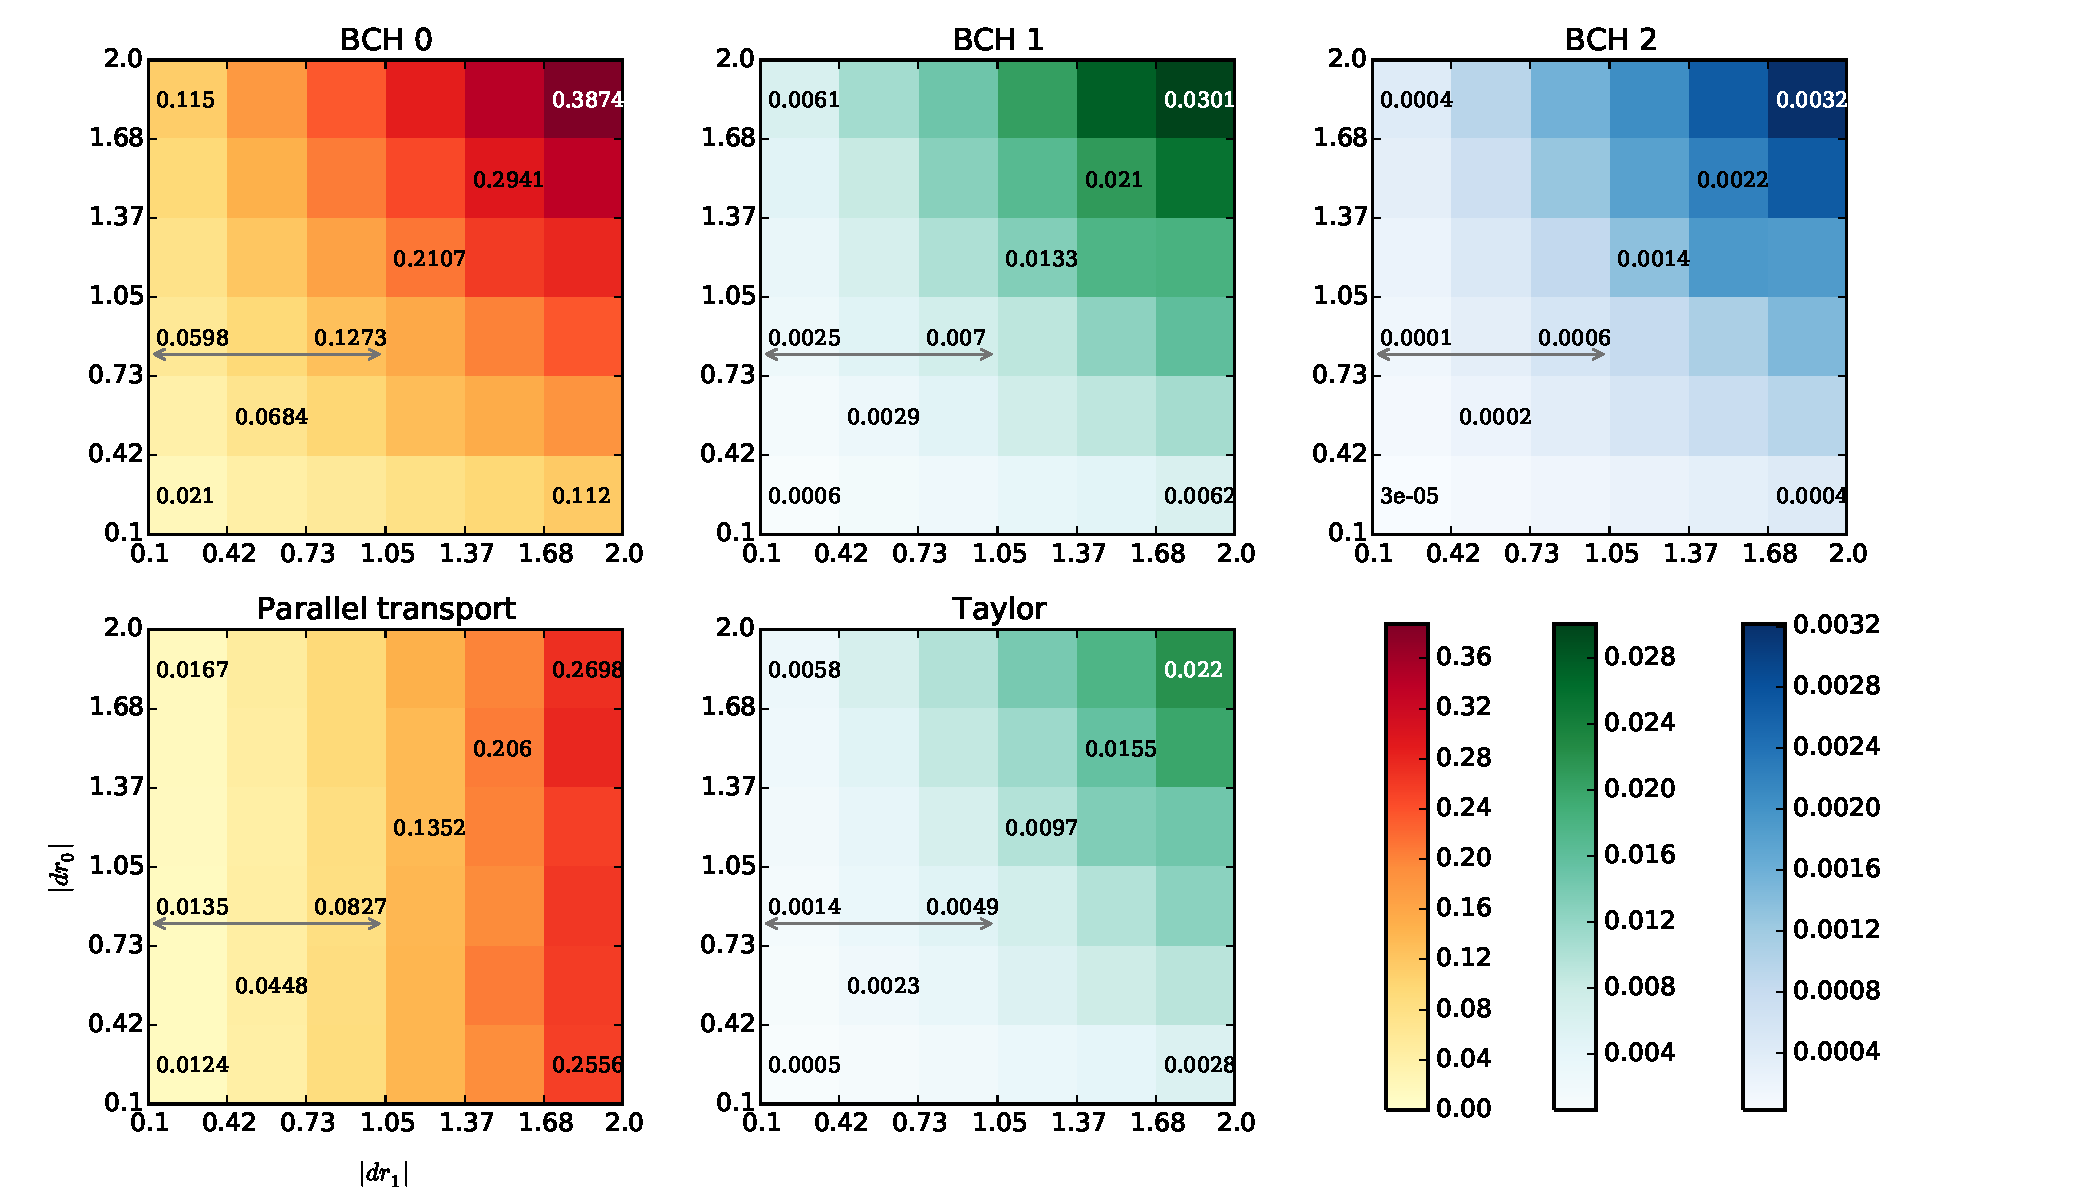
\includegraphics[scale=0.50]{figures/se2_image_scale.pdf}
 	\caption{Comparison of the errors for each numerical method to compute the Log-composition $dr_{0} \oplus dr_{1}$ in $\mathfrak{se}(2)$. Truncated BCH of degrees 0,1,2, parallel transport method and Taylor method are considered for different values of the norm of $dr_{1}$ (x-axes) and norm of $dr_{0}$ (y-axes). 
 	The value of each square corresponds to the average error of 500 random samples in each of the 6 sub-intervals between $0.1$ and $2.0$. Errors with BCH 0 and parallel transport method are comparable, but the parallel transport method is not symmetric and has better performance when $dr_{1}$ is small. BCH 1 and Taylor are comparable as well and they are both symmetric, but the best performance in terms of approximation is the BCH 2. Values of the sub-square under the \emph{gray arrows} are shown in the boxplot \ref{fig:se2_image_scale} where variance, quartiles and outliers are visualized.
 	 }
 	\label{fig:se2_image_scale}
 \end{figure}
 %
% % % % % % % % % % % % % % % % % % % % % % % % % % % % % % % % % % % % % %
% % % % % % % % % % % % % % % % % % % % % % % % % % % % % % % % % % % % % % 
\subsection{Methods and Results}

To compare the errors the computation of the log-composition for the methods here presented, two sets of $3000$ transformations of elements in $\mathfrak{se}(2)$ are randomly sampled with increasing norms in the interval $[0.1, 2.0]$. This interval is divided into 6 segments delimited by $ I = \text{linspace}([0.1, 2.0], 7)$ and for each couple of subintervals $[I(n_0), I(n_0+1)]$, $[I(n_1), I(n_1+1)]$ two sets of $500$ transformations $\{ dr_{0}^{(j)}\}_{j=1}^{500}$, $\{ dr_{1}^{(j)} \}_{j=1}^{500}$ having norms belonging to the respective intervals are sampled:
\begin{align*}
j=1,...,500 \quad &\quad  n_0, n_1 = 0,...,5 \\
\euclideanMetric{dr_{0}^{(j)}}_{\text{fro}} &\in [I(n_0), I(n_0+1)] \\
\euclideanMetric{dr_{1}^{(j)}}_{\text{fro}} &\in [I(n_1), I(n_1+1)]  
\end{align*} 
If $N$ is one of the numerical methods presented in section \ref{se:rigid_body_transformations} for the computation of the log-composition - $\text{BCH}^{0}, \text{BCH}^{1}, \text{BCH}^{2}, \text{Tl}, \text{pt}$ - 
then the error between the ground truth and the approximation provided by one of these numerical methods is given by
\begin{align*}
\text{Error}(dr_{0},dr_{1},N) 
:= 
\euclideanMetric{dr_{0}^{(j_0)} \oplus dr_{1}^{(j_1)} 
- 
N(dr_{0}, dr_{1}) }_{\text{fro}} 
\end{align*}

In figure \ref{fig:se2_image_scale}, each of the figure corresponds to a different method and each of the grade scale is the value computed with the function:
\begin{align*}
f(n_0,n_1,N) 
=
 \mathbb{E}\Big(
  \{ 
  \text{Error}(dr_{0}^{(j)},dr_{1}^{(j)},N) 
  \}_{j=1}^{500}
  \Big)
\end{align*}
Where the norm of $dr_{0}^{(j)}$ belongs to the interval $[I(n_0), I(n_0+1)]$ and the norm of 
$dr_{1}^{(j)}$ belongs to $[I(n_1), I(n_1+1)]$, and where $\mathbb{E}$ is the mean value.\\
The data indicated by the gray arrows in each plot corresponds are showed in the box-plot \ref{fig:se2_boxplot}
%
\begin{figure}[!ht]
	\hspace{-1cm}
	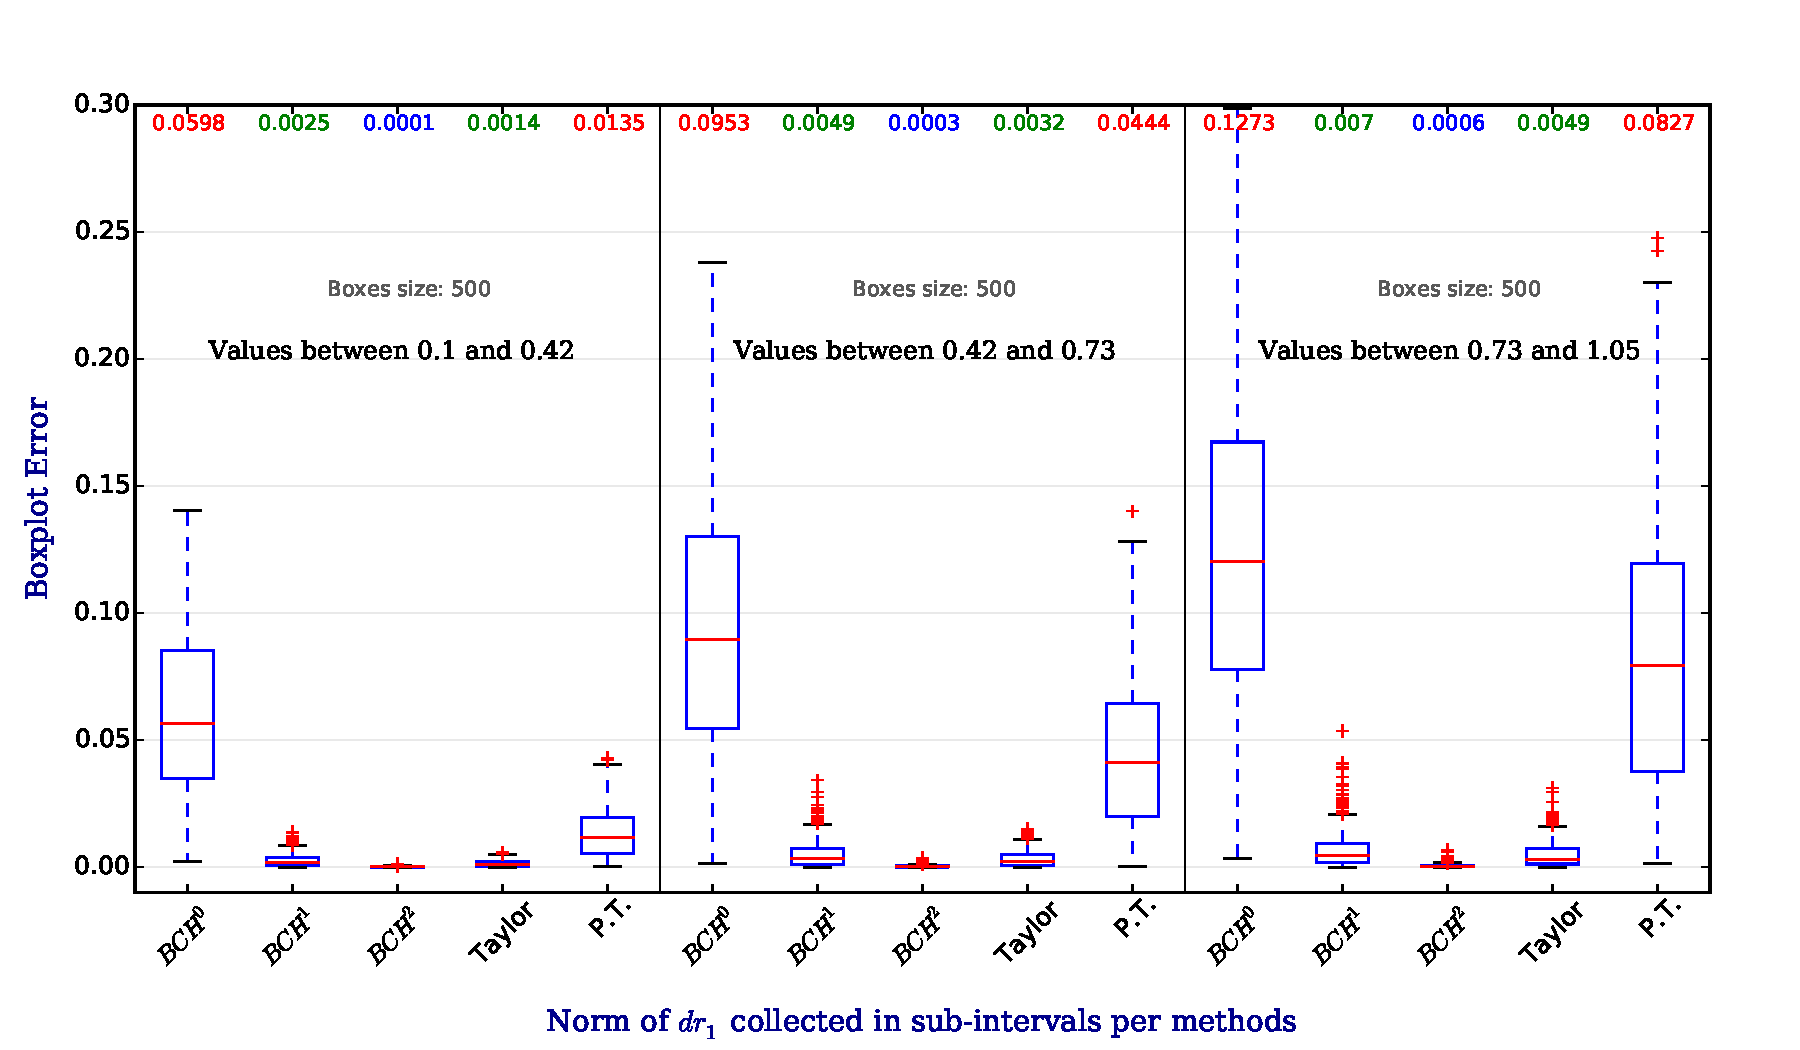
\includegraphics[scale=0.51]{figures/se2_boxplot.pdf}
	\caption{Errors of the numerical methods for the computation of the Log-composition of $dr_{0} \oplus dr_{1}$ in $\mathfrak{se}(2)$. Norm of $dr_{0}$ is in the interval $[0.37,1.05]$, norm of $dr_{1}$ in the interval $[0.1, 1.05]$ divided in 3 segments. Mean values of each box are shown in the first row in different colors. Shown data corresponds to a section of the image scale \ref{fig:se2_image_scale}, indicated by a gray arrow. As expected all of the error means increase with the of norm of $dr_1$, but the rate of the growth is different for each method.}
	\label{fig:se2_boxplot}
\end{figure}
%

From these results in $\mathfrak{se}(2)$ we can see that the second truncation error of the BCH formula provides the best result (the unit of measure is the same as the measure chosen for the translation or the rotation: it can be inches, cm, pixel, ...).

Method based on the $BCH^0$, that is utilized for example in the additive demons, do not involves any Lie bracket. Its results show that the bigger is the norm of the transformation involved, the bigger is its Lie bracket and its nested Lie bracket as appears in the $BCH^1$ and $BCH^2$. Do not take into account Lie brackets means do not take into account the curvature of the space \cite{misner1973gravitation}, whose significance is given by the experimental results. Parallel transport method tries to compensate the curvature using a geometrical approach considering different tangent spaces to the manifold of the transformation than the one at the origin. As expected from the formula is not symmetric. It provides better results than the $BCH^0$, and when the norm of $dr_1$ is small, results are close to the one obtained with $BCH^1$ when norms of $dr_0$ and $dr_1$ are below $1.3$.

Log-composition based on Taylor method has slightly better results than the $BCH^1$, but do not reach $BCH^2$, which provides the best results. This may be due to the fact that the Taylor belongs to $\mathcal{O}(dr_1^2)$ while the $BCH^2$ involves the Lie bracket $[dr_0,[dr_0, dr_1]] + [dr_1,[dr_1, dr_0]]$. Even if the truncated $BCH$ does not have a known asymptotic error (or big-O notation), this last observation provides that $BCH^2$ have a bigger asymptotic order of converges than $\mathcal{O}(dr_1^2)$, in $\mathfrak{se}(2)$.
%
\begin{figure}[!ht]
	%\hspace{0cm}
	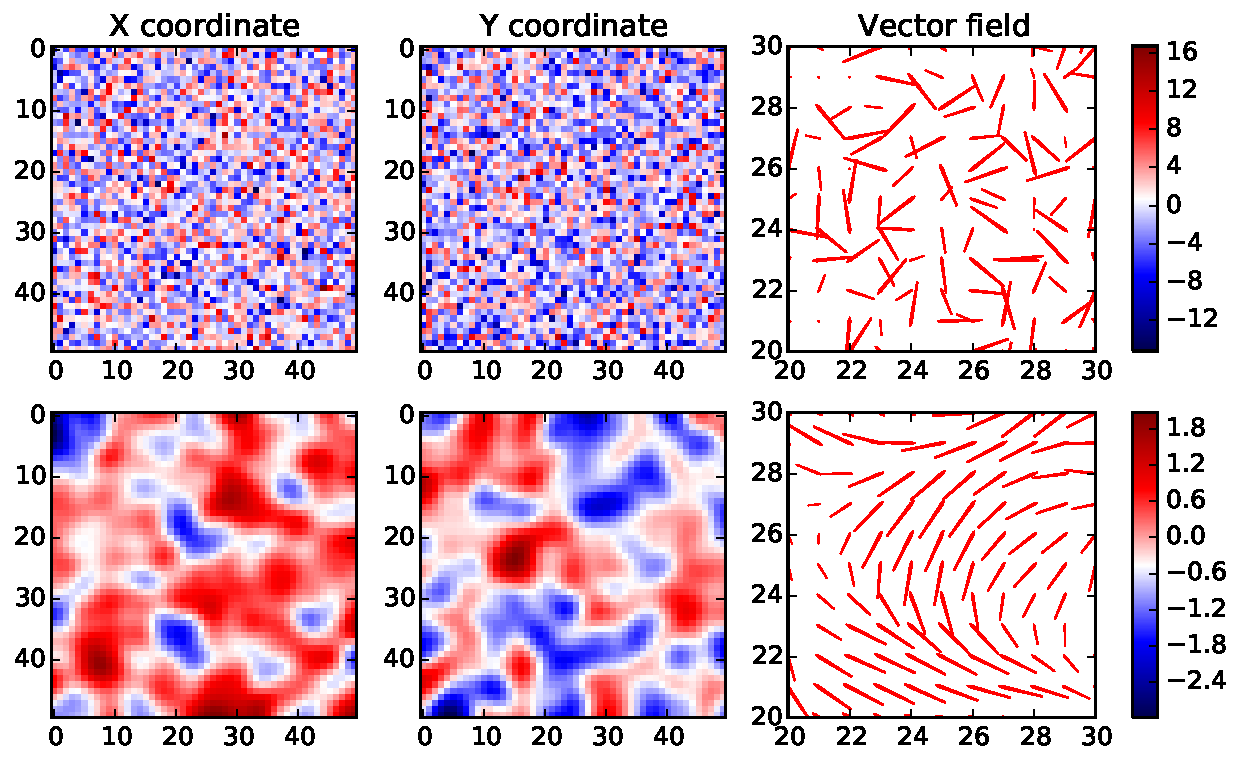
\includegraphics[scale=0.70]{figures/svf_gaussian_smoothing_effects.pdf}
	\caption{Random generated vector field before and after the Gaussian smoother: in the first row a random generated vector field of dimension $50\times 50 \times 2$ where the value at each pixel are sampled from a random variable with normal distribution of mean $0$ and sigma $4$. The second row shows the same random vector field after a Gaussian smoothing of sigma $2$ (the code is based on the scipy library ndimage.filters.gaussian\textunderscore filter). In the last column shows the quiver of the vector field in the squared subregion of size $10\times 10$ at the point $(20,20)$. From the colorscale it is also possible to see that the values distribution of the filtered image is not anymore symmetric. }
	\label{fig:SVF_gaussian_smoothing_effects}
\end{figure}

% % % % % % % % % % % % % % % % % % % % % % % % % % % % % % % % % % % % % %
% % % % % % % % % % % % % % % % % % % % % % % % % % % % % % % % % % % % % %
% % % % % % % % % % % % % % % % % % % % % % % % % % % % % % % % % % % % % % 
% % % % % % % % % % % % % % % % % % % % % % % % % % % % % % % % % % % % % % 
\section{Log-composition for SVF}
Before getting into the results for the log-composition of SVF it is important to spend some words about how random SVF are created and how to compare the norm of the approximation of $\mathbf{u}_0\oplus \mathbf{u}_1$ with the ground truth when this is not available.

% % % % % % % % % % % % % % % % % % % % % % % % % % % % % % % % % % % % % %
% % % % % % % % % % % % % % % % % % % % % % % % % % % % % % % % % % % % % % 
\subsection{Methods: random generated SVF.}
% How to generate a random SVF
A random generated SVF is a $5$-dimensional matrix with the structure presented in the equation \ref{eq:basic_data_structure}. 
The values of the dimensions are fixed while the values of the vectors are built in two phases. First of all, the value for each axis are randomly sampled from a normal distribution of mean zero and standard deviation $\sigma_{\text{init}}$. To introduce a correlation among each value, a Gaussian filter with standard deviation $\sigma_{\text{gf}}$ is then applied to regularize the values. In figure \ref{fig:SVF_gaussian_smoothing_effects} it is possible to see the effects of the two phases on a $50\times 50$ image.

\begin{figure}[!ht]
	\hspace{-1cm}
	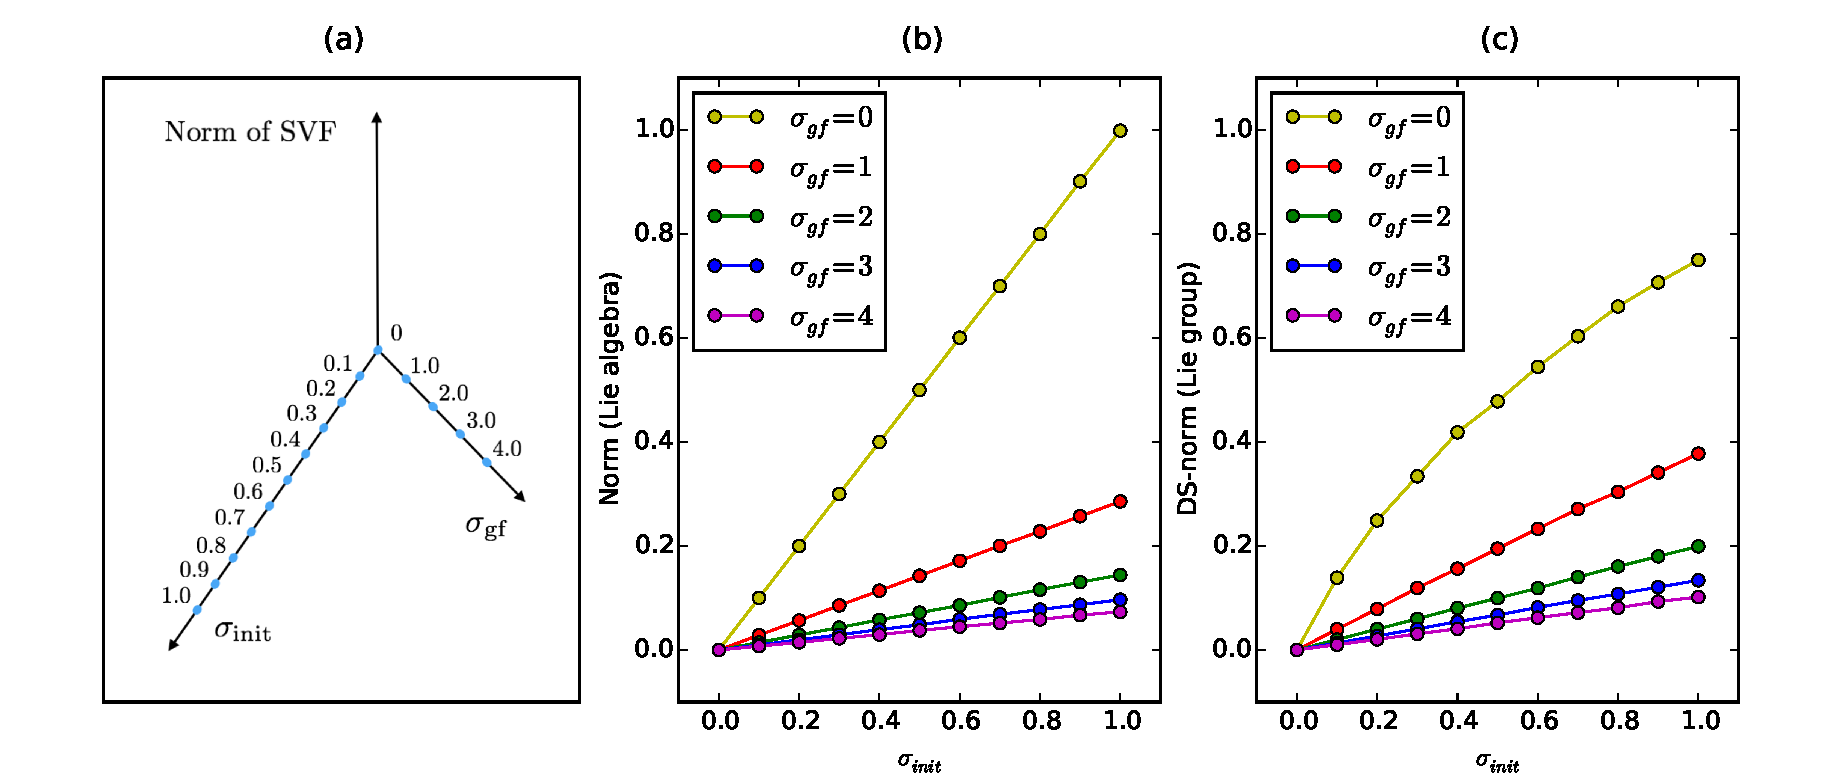
\includegraphics[scale=0.51]{figures/SVF_sigma_means_comparisons.pdf}
	\caption{Relationship between the initial standard deviation $\sigma_{\text{init}}$ that defines the random SVF (stationary velocity field), the standard deviation of the Gaussian filter $\sigma_{\text{gf}}$ utilized to regularize the SVF and its norm. Figure (a) represents schematically the two factors that define the norm of an SVF and with the blue dots we emphasized the values that has been chosen for the numerical computations proposed in (b) and (c). Figure (b) shows the mean of the norm of $10$ random generated SVF, as element of a Lie group, with initial standard deviation $\sigma_{\text{init}}$ (on the x-axis) and Gaussian filter with standard deviation $\sigma_{\text{gf}}$ (in different colors).
		Figure (c) shows the norm of the same element after exponentiating and so after having them in the Lie algebra.
		It is important to remark that it is not possible in general define a norm on a group. Nevertheless for matrices and for SVF it is possible to extend the norm from the Lie algebra to the Lie group, as proposed in chapter \ref{ch:spatial_transformations} with the definition of displacement field norm (DS-norm). }
	\label{fig:SVF_sigma_means_comparisons}
\end{figure}

% Norm defined in both Lie algebra and Lie group
The norm of a discretized SVF $\mathbf{u}$ is the one associated to the metric \ref{def:metric_two_svf} in the discretized case: $l^2$ instead of $L^2$ and on $\Delta\Omega$ discretization of the domain:
\begin{align*}
\euclideanMetric{\mathbf{u}}  
= 
\Big( \sum_{\mathbf{x} \in \Delta\Omega} \euclideanMetric{\mathbf{u}(\mathbf{x}) }_{l^2}^{2}  \Big)^{1/2}
\end{align*} 
and it coincides with the Frobenius Norm of the $5$-dimensional matrices $\mathbf{u}$.
When the SVF $\mathbf{u}$ is exponentiated in the Lie algebra $\exp(\mathbf{u}) = \varphi$, we have to rely on the fact that $\varphi - 1$ is a vector field whose norm can be computed with the discretization of \ref{def:metric_two_displacement_field}:
\begin{align*}
\euclideanMetric{\varphi}  
= 
\Big( \sum_{\mathbf{x} \in \Delta\Omega} \euclideanMetric{\mathcal{V}(\varphi)(\mathbf{x}) }_{l^2}^{2}  \Big)^{1/2}
=
\Big( \sum_{\mathbf{x} \in \Delta\Omega} \euclideanMetric{\varphi(\mathbf{x}) - \mathbf{x} }_{l^2}^{2}  \Big)^{1/2}
\end{align*} 
Where $\Delta\Omega$ is the discretized domain according to a grid.\\
To distinguish from the previous one, we called it DS-norm (displacement norm); as before, it coincides with the Frobenius norm of the $5$-dimensional matrices $\varphi - I$.

% Norm influenced by sigmas
Figure \ref{fig:SVF_sigma_means_comparisons} shows how the initial standard deviations $\sigma_{\text{init}}$ that defines the SVF are related with their norm before and after the exponentiation for $5$ different choices of the value of the standard deviation of the Gaussian filter $\sigma_{\text{gf}}$.
Except for the extreme case in which $\sigma_{\text{gf}} = 0$, that does not represent any SVF, we can see that an element in the Lie algebra $\mathbf{u}$ has a bigger norm of the correspondent in the Lie group. Moreover in both algebraic structure the norm shows a linear increasing trend of the norm with the increase of $\sigma_{\text{init}}$. An increase in $\sigma_{\text{gf}} $ implies a decrease in the slope of the trend. Also in this case the slope decreases regularly with an exponential model. 

% Slopes formulae
The linear regression of the model for each $\sigma_{\text{gf}}$ are given, in Cartesian coordinate by:
\begin{align}\label{eq:angular_coefficients_for_the_gf}
y = m_{\text{alg}}( \sigma_{\text{gf}} )x \qquad  \sigma_{\text{gf}} \geq 0
\qquad
\qquad
y = m_{\text{grp}}( \sigma_{\text{alg}} )x \qquad  \sigma_{\text{alg}} \ge 0
\end{align}
Where we indicated with $m_{\text{alg}}$ and $m_{\text{grp}}$ angular coefficients for the results obtained in the Lie group and in the Lie algebra respectively. They follow an exponential model, given by
\begin{align}
m_{\text{alg}}( \sigma_{\text{gf}} )
=
\alpha_0 e^{-\beta_0 \sigma_{\text{gf}}} + \gamma_0 
\qquad
m_{\text{grp}}( \sigma_{\text{gf}} )
=
\alpha_1 e^{-\beta_1 \sigma_{\text{gf}}} + \gamma_1
\end{align}
Where the parameters $\alpha_i, \beta_i, \gamma_i$ for $i=1,2$ can be computed numerically using an exponential regression algorithm.
\begin{center}
	\begin{tabular}{ c  c c c c c}
	$\alpha_0$ & $\beta_0$ & $\gamma_0$ & $\alpha_1$ & $ \beta_1$ & $\gamma_1$ \\
	0.91422836 &  1.48548466 &  0.08393943 &  0.67302265 &  0.82680977 &  0.07765811
	\end{tabular}
\end{center}
These values will be useful when we will need to compute $\sigma_{\text{init}}$ for a given $\sigma_{\text{gf}}$, when expecting a certain value of the norm of the SVF.

\begin{figure}[!ht]
	\hspace{-2.1cm}
	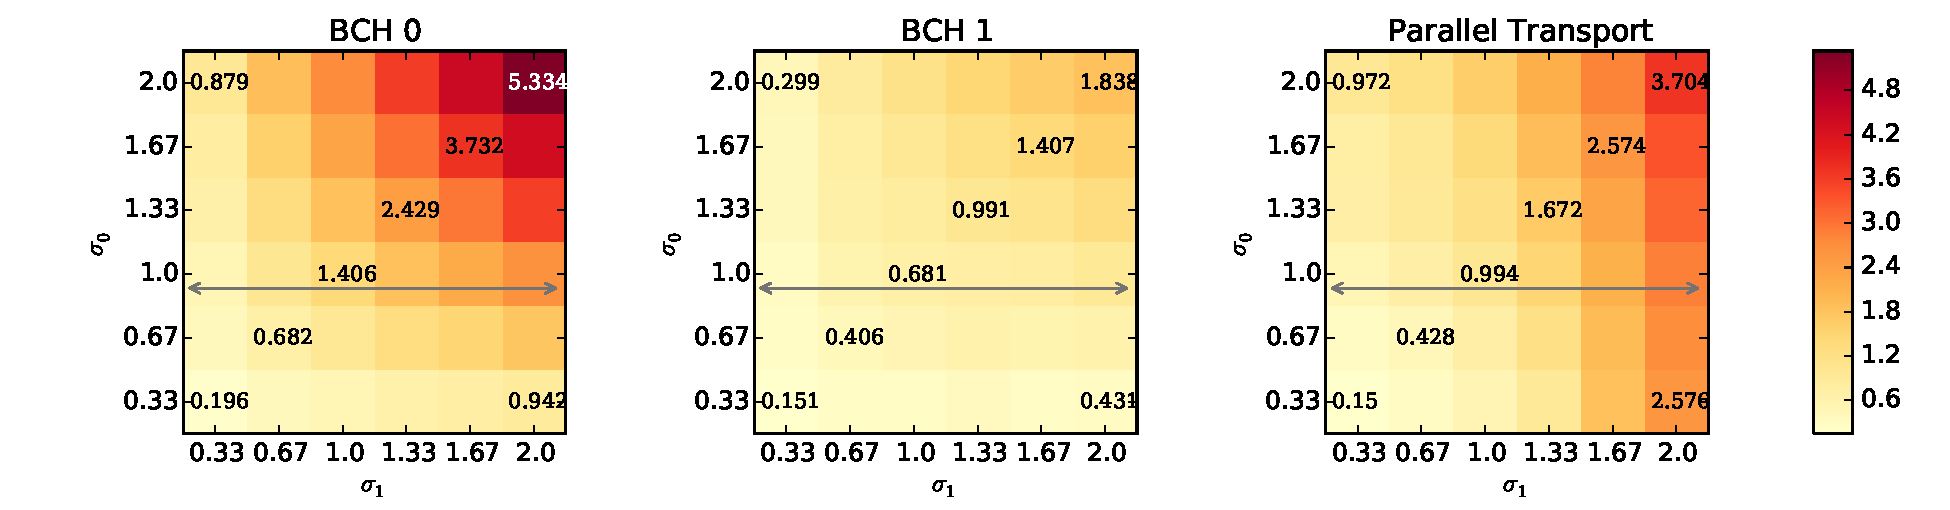
\includegraphics[scale=0.55]{figures/SVF_image_scale.pdf}
	\caption{Mean errors for the numerical computation of the Log-composition of randomly generated stationary velocity fields (SVF). Initial standard deviations of the SVF $\sigma_{\text{init}}^{0}$ and $\sigma_{\text{init}}^{1}$ are given by the values on the axis for each sampling of $15$ elements. The error is computed without a ground truth according to the formula \ref{eq:error_svf_sythetic_data}. When the norm of $\mathbf{u}_1$ is small (see figure \ref{fig:SVF_sigma_means_comparisons} to infer the norm from the standard deviations), parallel transport method and truncated BCH of degree 1 have comparable results, but parallel transport, as expected from the formula, is not symmetric respect to the size of the input vectors. Results of another sampling with the value of $\sigma_{\text{init}}^{0}$ and $\sigma_{\text{init}}^{1}$ are shown in figure \ref{fig:SVF_scatter_plot}.}
	\label{fig:SVF_image_scale}
\end{figure}

% Conclusion for the presentation of the random SVF
After showing how a random SVF is generated by the parameters $\sigma_{\text{init}}$ and $\sigma_{\text{gf}}$, and what is the relationship between the parameters and the resulting norm in both Lie algebra and Lie group, we can move toward the results of the numerical method for the log-composition obtained with these objects.

\begin{figure}[!ht]
	\hspace{-1.5cm}
	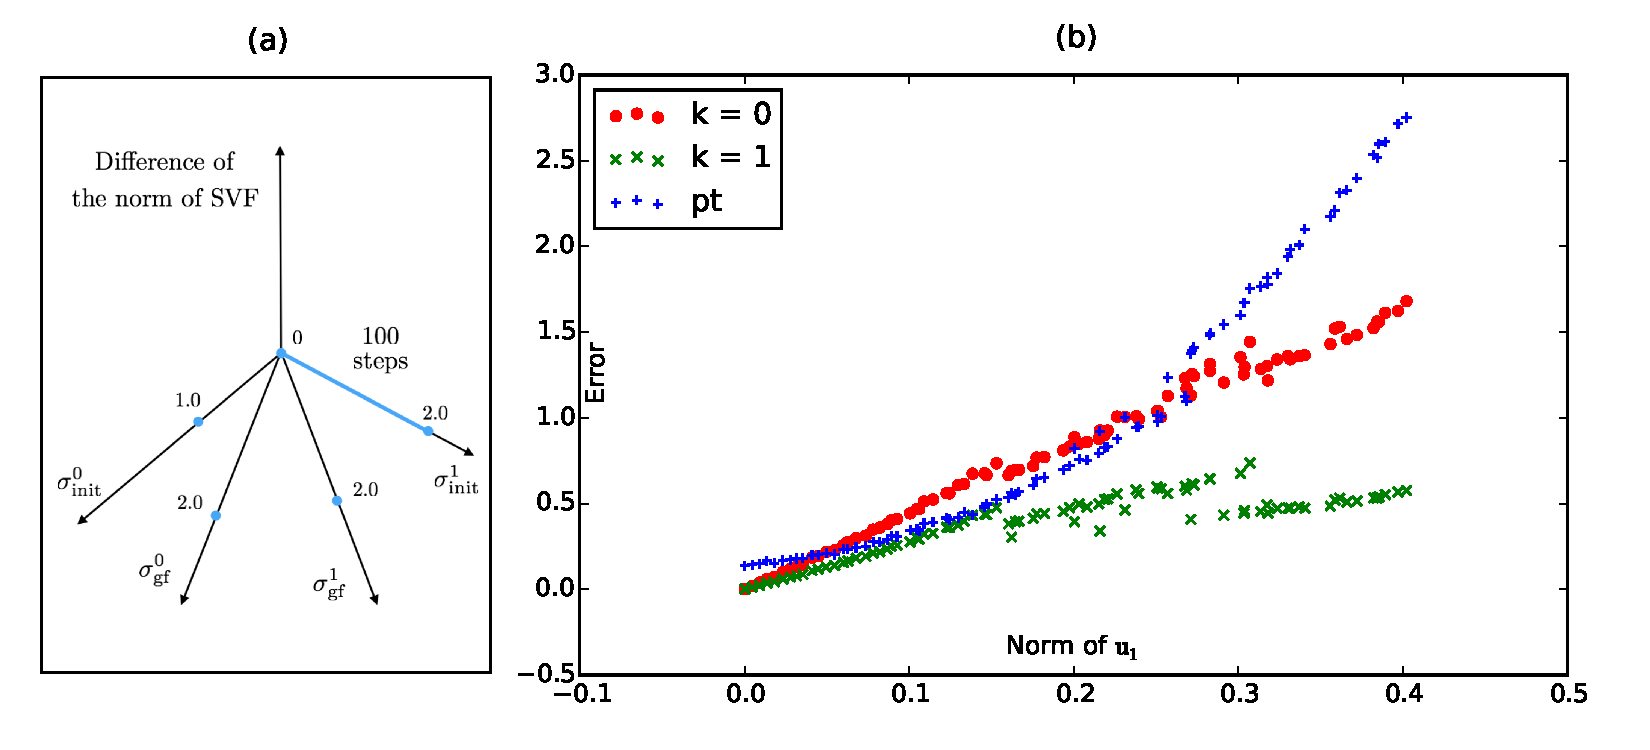
\includegraphics[scale=0.6]{figures/SVF_scatter_plot.pdf}
	\caption{Comparisons of the errors of numerical computation of $\mathbf{u}_0\oplus \mathbf{u}_1$ with the method of truncated BCH of degree 0,1 and parallel transport. Parameters' values of the random generated SVF are schematically represented in figure (a). A first set of $100$ SVF, that appears as first element in the log-composition, are generated with fixed parameters $\sigma_{\text{gf}}^{0} = 2.0$ and $\sigma_{\text{init}}^{0} = 1.0$; a second set of $100$ SVF, that appears as second element in the log-composition, are generated with the parameters $\sigma_{\text{gf}}^{1} = 2.0$ and $\sigma_{\text{init}}^{1}$ uniformly scattered in the the interval $(0.0, 2.0)$. On the x-axis fo figure (b) is shown the value of the resulting norm of $\mathbf{u}_1$ for the chosen parameters. On the y-axes the errors for the numerical computation of the Log-composition  }
	\label{fig:SVF_scatter_plot}
\end{figure}
%\begin{figure}[!ht]
%	\hspace{-1.5cm}
%	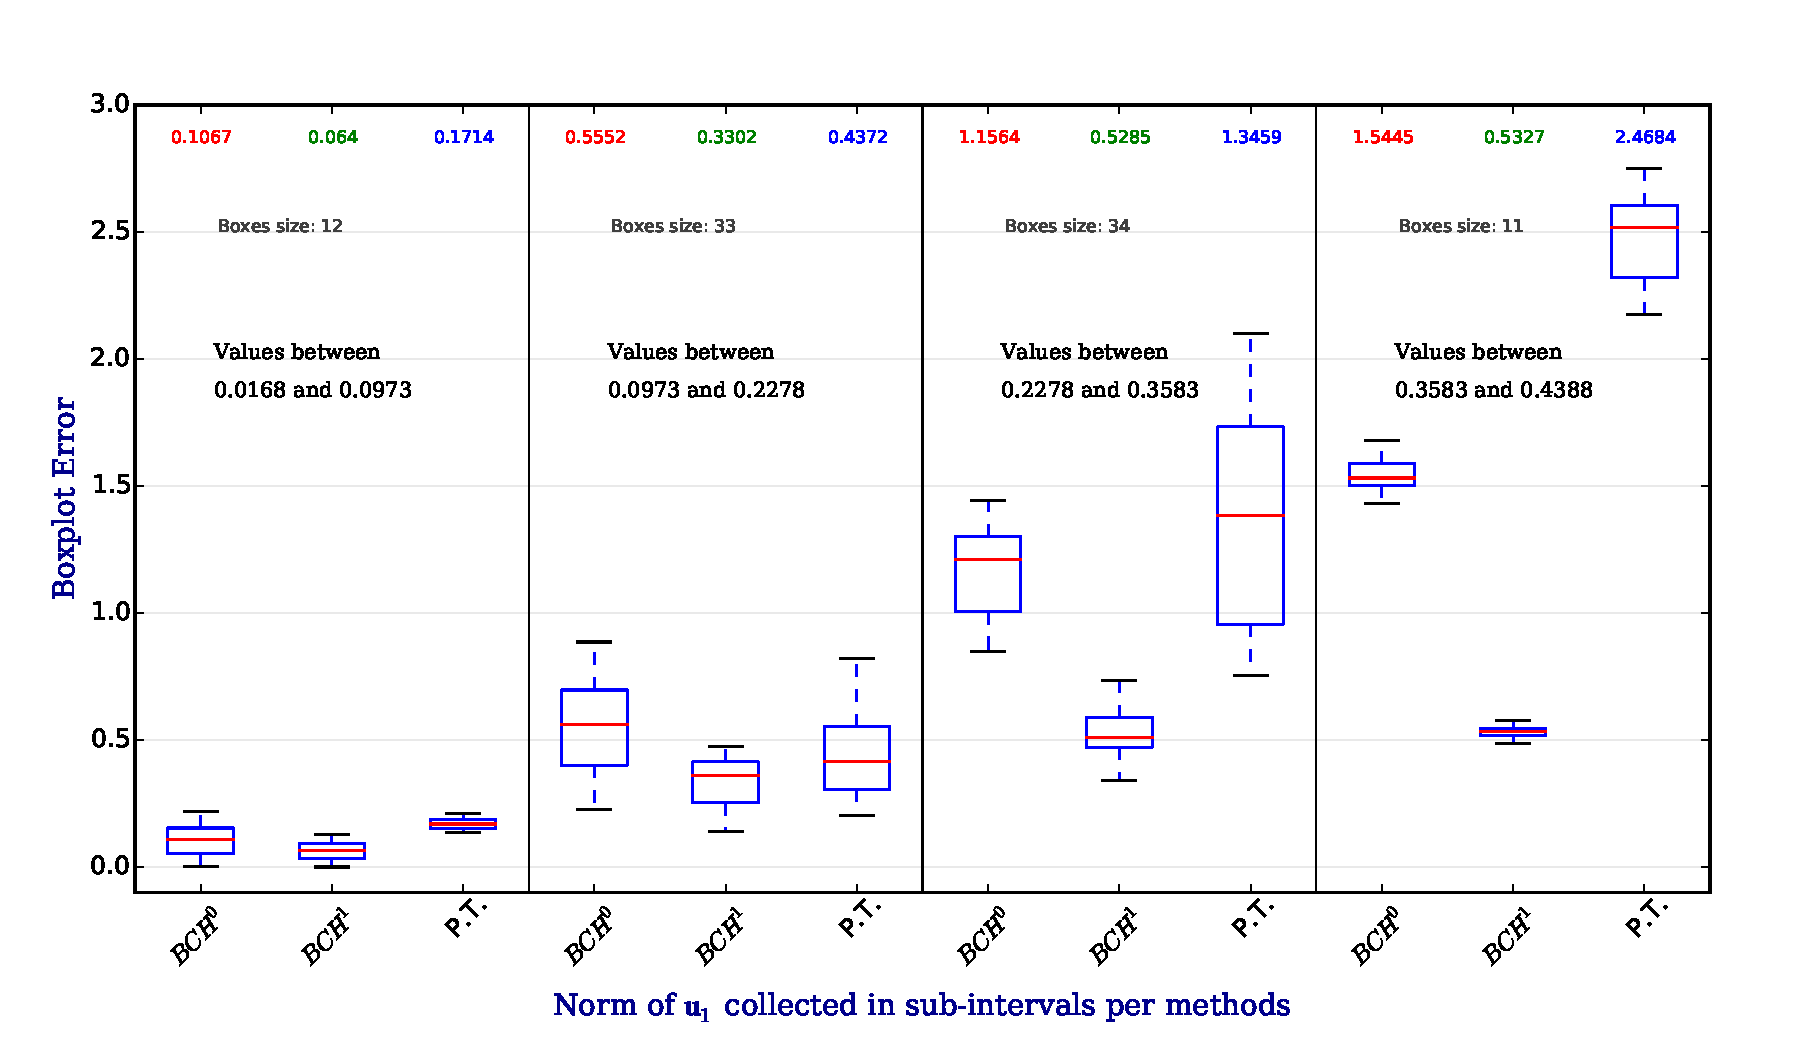
\includegraphics[scale=0.5]{figures/SVF_boxplot.pdf}
%	\caption{Log-composition for SVF computed using numerical methods of truncated BCH of degree 0,1 and parallel transport, represented in a boxplot.}
%	\label{fig:SVF_boxplot}
%\end{figure}

% % % % % % % % % % %% % % % % % % % % % %
% % % % % % % % % % %% % % % % % % % % % % % % % % % % % % % %
\subsection{Log-composition for synthetic SVF}
% which norm?
In figure \ref{fig:SVF_image_scale} we present the results of the numerical computation of the log-composition $\mathbf{u}_0\oplus\mathbf{u}_1 = \log(\exp(\mathbf{u}_0)\circ \exp(\mathbf{u}_1))$. Despite the lack of a ground truth for the SVF, given $\mathbf{u}_0$ and $\mathbf{u}_1$ in the Lie algebra we can compare the numerical approximation of $\mathbf{u}_0\oplus\mathbf{u}_1$ after exponentiating, with $\exp(\mathbf{u}_0)\circ \exp(\mathbf{u}_1)$. The norm utilized is the one proposed in the equation \ref{def:metric_one_svf_one_displacement_field}:
\begin{align}
\text{Error}_{\oplus}(\mathbf{u}_0, \mathbf{u}_1)
= 
\Big(\int_{\Omega} \euclideanMetric{\mathcal{V}(\exp(\mathbf{u}_0\oplus\mathbf{u}_1)) - \mathcal{V}(\exp(\mathbf{u}_0)\circ \exp(\mathbf{u}_1))}_{L^2}^{2} d\mathbf{x} \Big)^{1/2}
\end{align} 
that, when discretized become
\begin{align}\label{eq:error_svf_sythetic_data}
\text{Error}_{\oplus}(\mathbf{u}_0, \mathbf{u}_1) 
= 
\Big( \sum_{\mathbf{x} \in \Delta\Omega} 
\euclideanMetric{\exp(\mathbf{u}_0\oplus\mathbf{u}_1)(\mathbf{x}) 
	-
\big(\exp(\mathbf{u}_0)\circ \exp(\mathbf{u}_1)\big)(\mathbf{x}) 
	  }_{l^2}^{2}  \Big)^{1/2}
\end{align} 
For the unknown analytical value of $\mathbf{u}_0\oplus\mathbf{u}_1$ the error of the above equation is $0$. When we use one of the introduced numerical method we obtain the results presented in figure \ref{fig:SVF_image_scale} and \ref{fig:SVF_scatter_plot}. The limitation of this strategy to compute the error of the numerical method without a ground truth is that it is based on the numerical algorithm utilized for the computation of the Lie exponential. In this case we utilized the scaling and squaring proposed in \cite{arsigny2006log}. This limitation may eventually not bias the results, since the scaling and squaring is utilized it the both sides of the difference in the computation of the error, therefore we expect that this numerical approximation do not biasing the results unbalancing one side over the other.

% figures presentation and comment to general results.
In figure \ref{fig:SVF_image_scale}, we can see the difference between the numerical methods based on $\text{BCH}^0$, $\text{BCH}^1$ and parallel transport. To each square correspond the mean of $15$ log-compositions between the SVF $\mathbf{u}_0$ and $\mathbf{u}_1$ randomly generated with $\sigma_{\text{init}}^{0}$ and $\sigma_{\text{init}}^{1}$ equals to one of the value in the array $(0.33, 0.67, 1, 1.33, 1.37, 2.0)$. The standard deviation of the Gaussian filter $\sigma_{\text{gf}}^{0}$ and $\sigma_{\text{gf}}^{1}$ are constant and equal to $2.0$. As previously noticed for matrices, the method based on the truncated  BCH are symmetric while the same does not happen for the parallel transport. 

A more detailed analysis on the subinterval indicated by the gray arrow on the figure \ref{fig:SVF_image_scale}, is shown in \ref{fig:SVF_scatter_plot}.
Here we can see that for SVF the numerical method based on parallel transport is never better than  truncated BCH of order $1$ (green x) and provides worst results than the simple sum in the truncated BCH of order $0$ (red circle) when the norm is greater than $0.35$ (with a much higher computational cost). It is also true that for small value the performance of the parallel transport method is below the line draw by the red circles and it is tangential to the green one.

% introduction of the next section
In the results previously showed we can notice some notable absents: non of the method for the numerical computation of the log-composition based on truncated BCH of order greater than $1$ has been proposed. The reason of this is explained in the next section.


% % % % % % % % % % % % % % % % % % % % % % % % % % % % % % % % % % % % % %
% % % % % % % % % % % % % % % % % % % % % % % % % % % % % % % % % % % % % % 
\subsection{Truncated BCH formula: The problem of the Jacobian matrix.}\label{se:jacobian_problem}

% why we will take into account only the BCH 0 and the BCH 1 methods.
% Theoretical problems: that the Jacobian is utilized in the Lie bracket from Marcos' paper
The use of the truncated BCH for the numerical approximation fo the log-composition is problematic for SVF. As shown in figure \ref{fig:se2_image_scale}, i the finite dimensional case the truncated BCH of degree $2$ provides the best results over the Taylor method and the parallel transport method. In the infinite dimensional case the truncated BCH involves the Jacobian matrix, that is problematic by a numerical point ov view.

\begin{figure}[!ht]
	\hspace{0cm}
	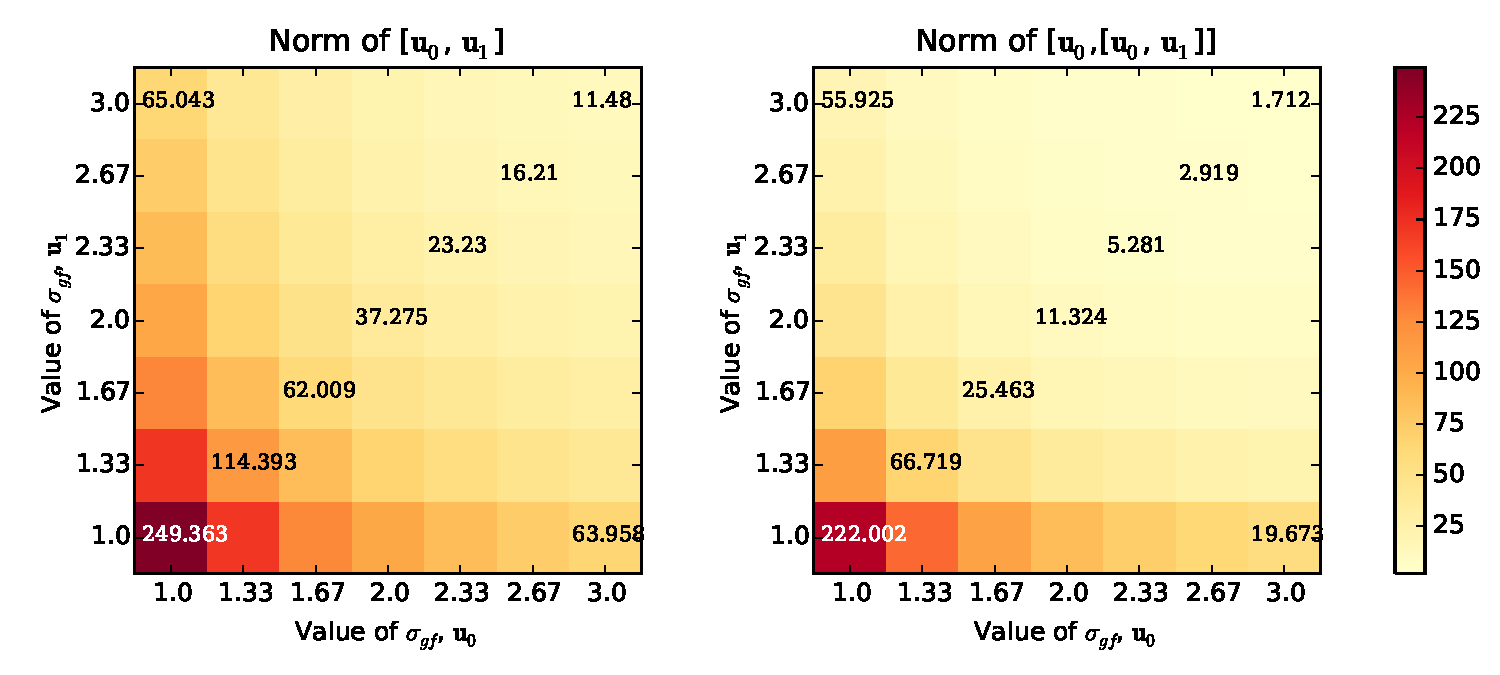
\includegraphics[scale=0.5]{figures/SVF_image_scale_bracket_versus_gaussian.pdf}
	\caption{Relationship between the standard deviation of the Gaussian smoother that generates the SVF and the norm of the Lie bracket. Each square contains the means of $10$ Lie bracket (left) or nested Lie bracket (right) generated with initial standard deviation equals to $2$ and standard deviation of the gaussian smoother $\sigma_{\text{gf}}$ indicated on the axes.}
	\label{fig:SVF_image_scale_bracket_versus_gaussian}
\end{figure}

% 2 limitation of the JACOBIAN. Image scale figure
On one side every time the differentiation of a vector is required (usually computed with finite difference method -reference-), the results is unstable and sensitive to noise. On the other side, in figure \ref{fig:SVF_image_scale_bracket_versus_gaussian} we can see that the smoother are the SVFs involved in the log composition, the smaller is the norm of the resulting Lie brackets. Therefore, for a couple of very smooth stationary velocity field, the higher term of the BCH carry little or not information.

% Boxplot comment, why it behave in this way
For both of these reasons it follows that an increase in the degree of the truncated BCH does not necessarily implies a better approximation or an increase in the robustness of the method. Looking at the boxplot in figure \ref{fig:SVF_boxplot_comparisons_BCH} we can see why in the previous section we did not compare the truncated BCH of order higher than 1 with the parallel transport method. The truncated BCH of higher degrees does not have better results than the degree 1. It is also interesting to notice that in some cases the truncated BCH formula of degree 2 provides worst results than the truncated BCH formula of degree 1, in particular when the involved SVF have been generated with a small Gaussian smoother.

\begin{figure}[!ht]
	\hspace{-0.5cm}
	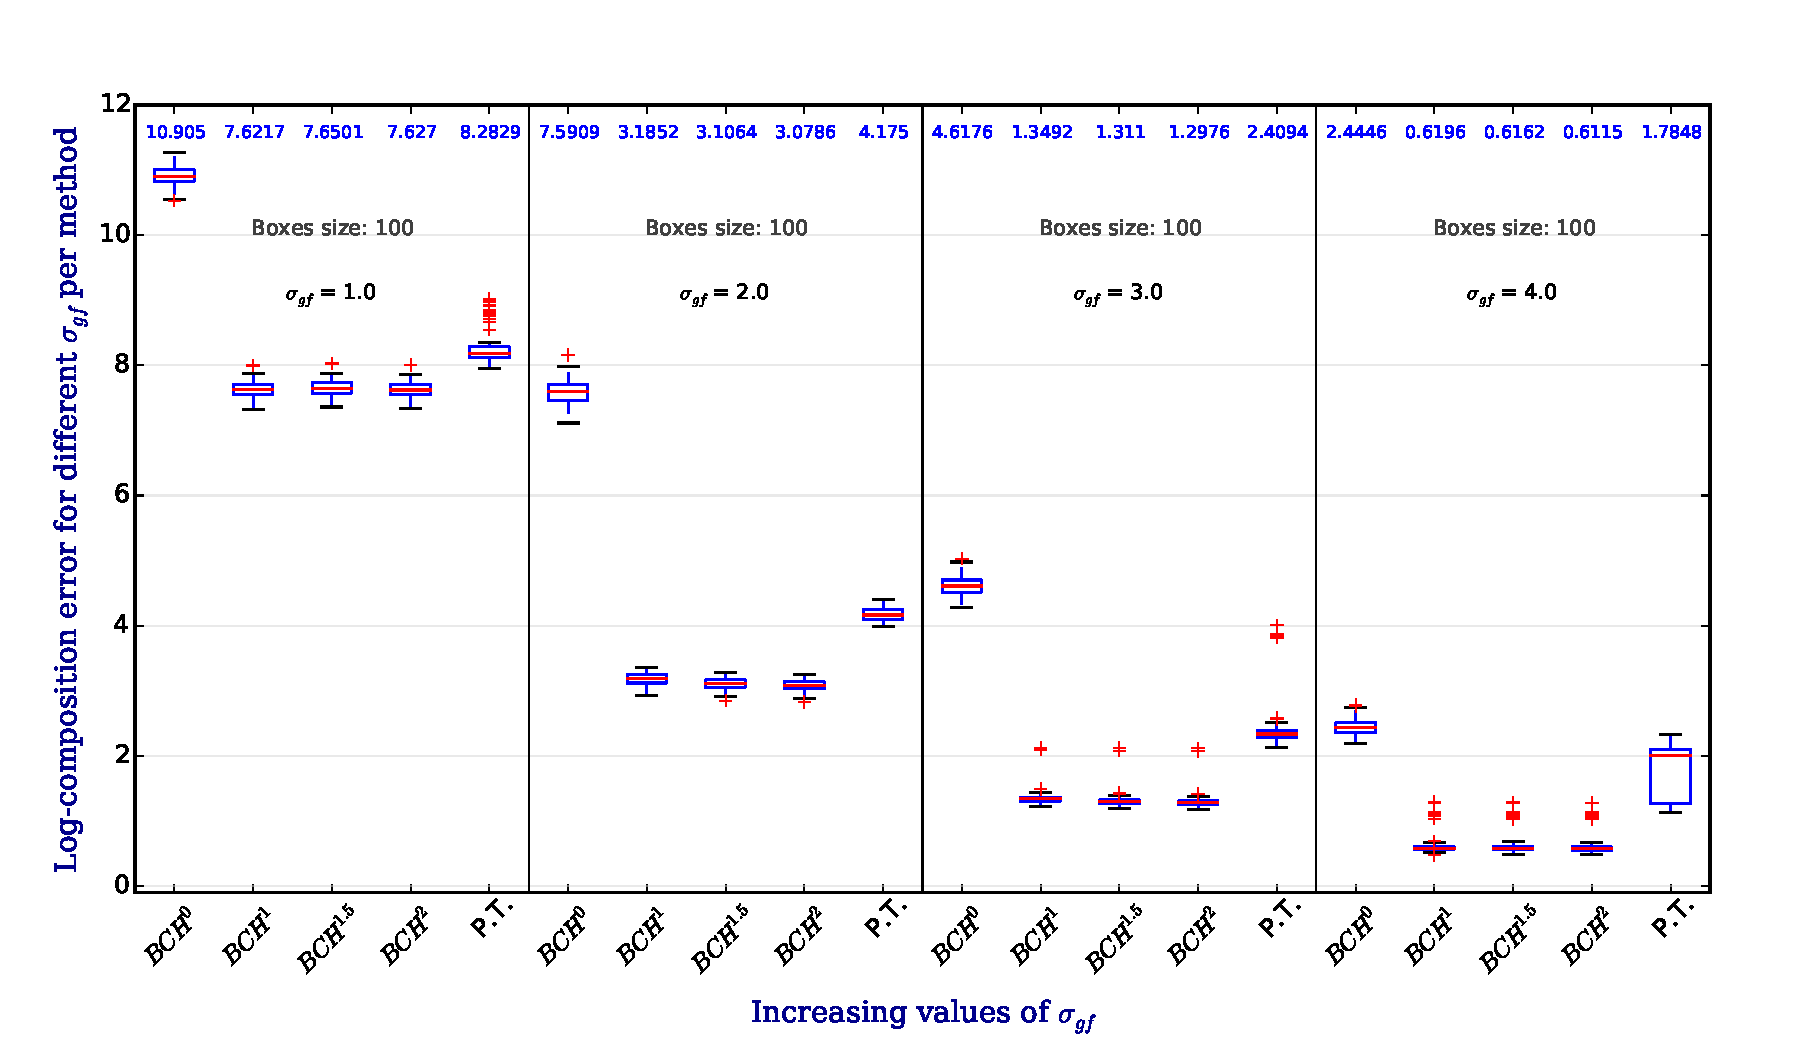
\includegraphics[scale=0.5]{figures/SVF_boxplot_comparisons_BCH.pdf}
	\caption{Boxplot to compare the error between truncated BCH methods of degree $0$, $1$, $1.5$ and $2$. The size of each box is $100$ and the approximation of $\mathbf{u}_{0}\oplus \mathbf{u}_1$ is performed with $\euclideanMetric{\mathbf{u}_{0}} = 1.0$ and $\euclideanMetric{\mathbf{u}_{0}} = 0.1$. The standard deviation of the Gaussian filter $\sigma_{\text{gf}}$ belongs to the set $(1.0, 2.0, 3.0, 4.0)$ and the initial standard deviation is computed such that $\sigma_{\text{init}} = \euclideanMetric{\mathbf{u}}/m_{\text{alg}}(\sigma_{\text{gf}})$ according to the formula \ref{eq:angular_coefficients_for_the_gf}. With this strategy we have been able to compare vector of constant norm generated with increasing values for $\sigma_{\text{gf}}$. The numbers written in blue above each box represents the mean value of the errors. For small $\sigma_{\text{gf}}$, an increase in the order of the approximation does not always corresponds to a decrease in the error, and in general there no great improvements can be registered when the degree is greater than 1. }
	\label{fig:SVF_boxplot_comparisons_BCH}
\end{figure}


\newpage
% Conclusions for syntetic data: where are the errors and why we are moving towards the real data.
% Why going toward real svf, 

% % % % % % % % % % % % % % % % % % % % % % % % % % % % % % % % % % % % % %
% % % % % % % % % % % % % % % % % % % % % % % % % % % % % % % % % % % % % % 
\section{A Problem for Three Brains} % {A three-brain problem}
The experiments performed on synthetic data provides important informations to validate and compare the methods, but gives little or no information of what may happen in the real cases. 

To obtain a validation for the real cases, the most natural way would be embed the method in a diffeomorphic demon registration algorithm and compare its results with the different versions of the log-composition implemented for the computation of the update.

But, since the log-composition is only a small piece of the registration algorithm, it may be difficult to understand to what extent the change of the numerical method for the log-composition would impact the results and what is due to other part that play a more important role (as the optimization strategy) in the registration algorithm.

For our purposes we design an experiment that involves three brains... 


% % % % % % % % % % % % % % % % % % % % % % % % % % % % % % % % % % % % % %
% % % % % % % % % % % % % % % % % % % % % % % % % % % % % % % % % % % % % % 
% % % % % % % % % % % % % % % % % % % % % % % % % % % % % % % % % % % % % % 
\section{Log-Algorithm for SVF}

To compare the different numerical methods for the the logarithm computation algorithm we remain where a ground truth is available, i.e. in the finite dimensional case. We consider a data set of $200$ random matrices in the Lie group $SE(2)$ with their respective logarithm in $\mathfrak{se}(2)$ computed using the closed form presented in chapter \ref{ch:spatial_transformations}. For each of the method considered and for each of the random matrix we have convergence up to a precision of $10^{-12}$ before the $50^{\text{th}}$ iteration.

In figure \ref{fig:log_computation_boxplot} we can see the average number of iterations required to reach the solution with a precision of $10^{-4}$ for each of the numerical method considered. Each box represents $200$ random matrices in $SE(2)$ with Frobenius norm uniformly selected between $1$ and $3$.

As obtained in the log-composition the results obtained with parallel transport is comparable with the one obtained with the truncated BCH of degree $1$. Remarkably, in this case, an increase in the degree of the truncated BCH does not ensure a faster convergence and the Taylor method, provides the slower algorithm. The reason for these facts are not clear are the moment and are worthed to be investigated in a future work.

\begin{figure}[!ht]
	\hspace{-0.5cm}
	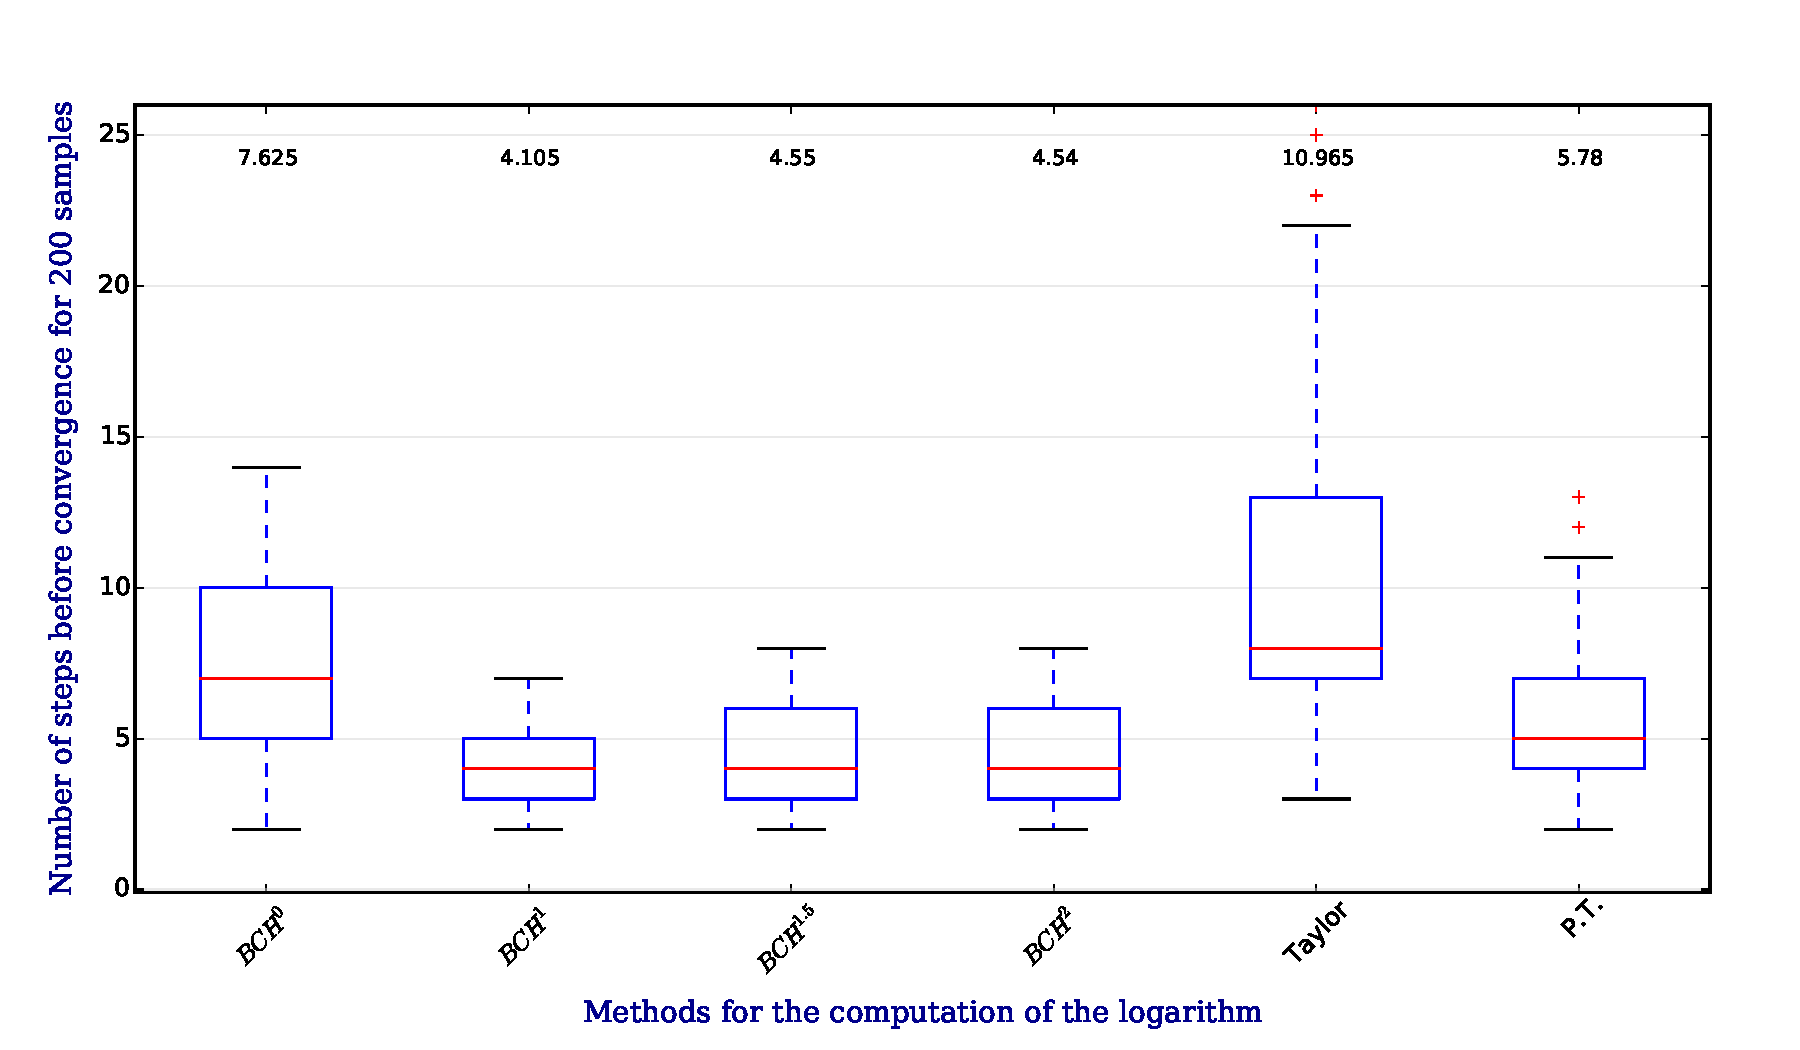
\includegraphics[scale=0.5]{figures/log_computation_boxplot.pdf}
	\caption{Number of steps required to obtain convergence in for different methods utilized in the logarithm computation algorithm. The data set contains $200$ random matrices in the Lie group $SE(2)$, with Frobenius norm between $1$ and $3$. On the top it is possible to visualize the mean number of step to reach the convergence for each method.}
	\label{fig:log_computation_boxplot}
\end{figure}


% % % % % % % % % % % % % % % % % % % % % % % % % % % % % % % % % % % % % %
% % % % % % % % % % % % % % % % % % % % % % % % % % % % % % % % % % % % % % 
\section{Empirical Evaluations of the Computational Time}

For the finite dimensional case, a dataset of $36000$ random generated matrix with norm between $0.0$ and $2.0$ has been utilized to measure the computational time of each of the numerical method for the computation of the log-composition here presented. Sum of the computational time for the whole data set is give in seconds, in the following table:\\

\hspace{-1cm}
\begin{tabular}{ c | c | c | c | c | c | c }
Ground & $\text{BCH}^0$ & $\text{BCH}^1$ & $\text{BCH}^{1.5}$ & $\text{BCH}^2$ & Taylor & p.t. \\
\hline
1.07402015 & 0.18845153 & 0.57751322 & 1.24413943 & 1.78752184 & 0.77354765 &
2.26586294 
\end{tabular}
\vspace{0.5cm}

The first column provides the computation of the ground truth, i.e. the closed for the computation of $dr_0 \oplus dr_{1}$. We can see that the computation of the $\text{BCH}^0$ is the fastest, since it consists only in a sum, while the computation of the parallel transport is four time slower than the $\text{BCH}^1$.

When dealing with SVF, the computational time strongly depends on the size of the vector field involved. In figure \ref{fig:svf_computational_time} we can see the relation between the size of the vector field and the increase in the computational time for a data set of $20$ random generated SVF.

\begin{figure}[!ht]
	%\hspace{-0.5cm}
	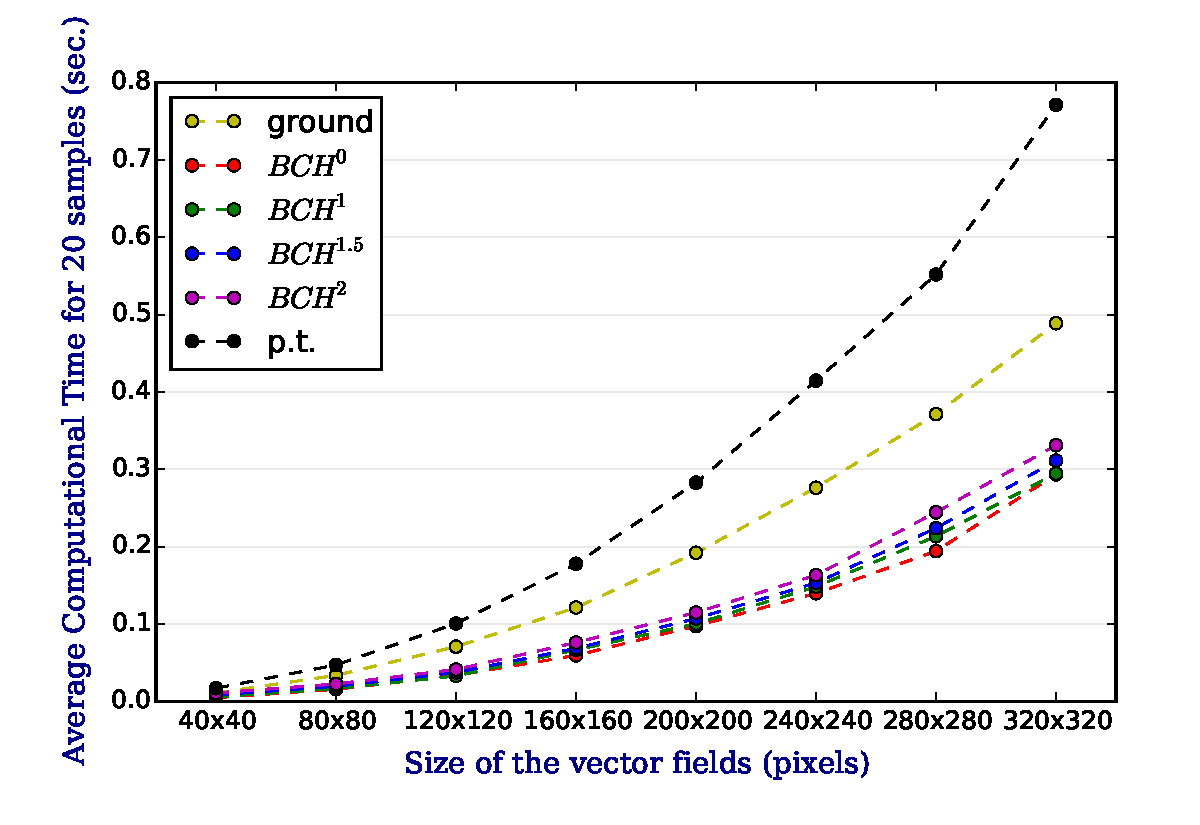
\includegraphics[scale=0.7]{figures/svf_computational_time.pdf}
	\caption{Relationship between the size of the figure (x-axes) and the computational time for a data set of $20$ random generated SVF. The yellow line labeled with ground represents the time of the computation of $\exp{\mathbf{u}_0}\circ \exp{\mathbf{u}_1}$, while the other represents the exponentiation of the numerical method for the computation of the log-composition.}
	\label{fig:svf_computational_time}
\end{figure}

% % % % % % % % % % % % % % % % % % % % % % % % % % % % % % % % % % % % % %
% % % % % % % % % % % % % % % % % % % % % % % % % % % % % % % % % % % % % %
% % % % % % % % % % % % % % % % % % % % % % % % % % % % % % % % % % % % % % 
\section{Conclusions}\label{se:conclusions}

% the log-composition battezzata per nome in vista della sua utilita' pratica. Presentata con il log-euclidean framework gia' proposto da Arsigny.

% Framework that justifies the use of the frobenius provided improperly a norm for the the SVF.

% discuraging the use of the truncated BCH for SVF
A seen from results not 


% Parallel transport method as possible valid alternative for the computation of the log-composition
Considering only the results, this one-year research can be considered much ado about nothing, but...\\
Computational time...!

% % % % % % % % % % % % % % % % % % % % % % % % % % % % % % % % % % % % % %
% % % % % % % % % % % % % % % % % % % % % % % % % % % % % % % % % % % % % % 
\section{Further Researches}\label{se:further_research}




The BCH is proved only when the exp and log can be expressed in power series, so when the Lie group and the Lie algebra involved belongs to the same bigger group. This is not the case of the infinite dimensional Lie group of diffeomorphisms,


% More tests on real data are necessarily

% More tests on diffeomorphic demon framework where parallel transport could fit sometimes better than the sum, and could avoid the use of the jacobian matrices.

% theoretical side in general
Starting from the definition of Lie log-group of diffeomorpshisms $(\mathfrak{g} , \oplus)$, to have an algebraic definition of this approximation, we can consider its quotient over the ideal generated by $(\text{ad}_{\mathbf{u}}^{m}, \text{ad}_{\mathbf{u}}^{n})$, which provides the group $(\quotient{\mathfrak{g}}{(\text{ad}_{\mathbf{u}}^{m}, \text{ad}_{\mathbf{u}}^{n})}, \oplus)$. Further investigations in this direction is not prosecuted.

% theoretical side for an improvement on the parallel transport: it has been shown that expoiting the fiber bundle on the Lie group works, for both matrices and SVF. But based on may assumptions. Investigating better the situation may lead to an improved formula for the computation of the log-composition.





